\section{Компьютерная имитация макроэкономических моделей} 

В рамках дипломной работы была разработана программа, которая эмулирует
биматричную игру на временных шкалах и доказывает эмпирически изложенные в
работе результаты.  

Разработка программного продукта велась на языке Python 3.4.
Программа позволяет пользователю задать $r^g$, $r^p$ и соответствующие
скалярные функции поведения игрока в определенный момент времени. Значениями
данной функции будет вероятность выбора игроком  стратегии $H$ в данный период
времени. Так же пользователь может задать количество запусков игры с входящими
данными для подсчета статистики. В качестве интерфейса входящих данных был
выбран простой текстовый файл, что позволяет строить в случае необходимости 
большие последовательности экспериментов.

\subsection{Анализ устойчивости стратегий в модели Барро-Гордона}
Положим, что матрица выигрышей двух игроков соответствует~\ref{table:sec:ot:real},
$r^g= 7$ (количество ходов правительства), $r^p= 4$ (количество ходов общества).

\begin{table}[h]
	\centering
	
	\caption{}	
			\footnotesize Матрица выигрышей для модели Барро-Гордона\\
			\normalsize
			
\begin{tabular}{|l|l|c|c|}
	\hline
	\multicolumn{2}{|l|}{\multirow{2}{*}{}} & \multicolumn{2}{l|}{Общественность} \\ \cline{3-4} 
	\multicolumn{2}{|l|}{}                  & L                & H                \\ \hline
	\multirow{2}{*}{Правительство}    & L   & 0, 0             & -1,-1            \\ \cline{2-4} 
	& H   & $\frac{1}{2}$,-1             & $-\frac{1}{2}$, 0            \\ \hline
\end{tabular}

	\label{table:sec:ot:real1}
\end{table}

Проверим выполнение условия теоремы~\ref{eq:sec:tech:theoremSystem} для матрицы выигрышей~\ref{table:sec:ot:real1}. 
$$
r^g> \bar{r^g}(R) = \left\{ 
\begin{aligned} 
&2r^p= 2r^p, &&\text{если } R=0
\\
&2(1+R)r^p= 2(1+R)r^p, &&\text{если } 	R\in\left(0; \frac{1}{2}\right)
\\
&2Rr^p= 2Rr^p, &&\text{если } 	R\in\left( \frac{1}{2};1\right)
\end{aligned}
\right.		
$$

$$
r^g> \bar{r^g}(R) = 0$$
$$
4 > 0
$$
Следовательно $\frac{r^g}{r^p} \in \left(\frac{3}{2};2\right)$ выбраны
правильно и все совершенные равновесия по под-играм должны быть совершенными
равновесиями по под-играм Рамсея. 
 
Рассмотрим случай, когда правительство скорее склонно ввести высокий уровень
инфляции, а общественность предполагая, что правительство пойдет на этот шаг с
высокой долей вероятности поднимет зарплаты.

Зададим распределение вероятностей выбора cтратегии $H$ для каждого из двух игроков:
 \begin{gather*}
 	q^g = \left[ 0.5; 0.9; 0.7; 0.5; 0.9; 0.73; 0.8 \right], \\
 	q^p = \left[ 0.8; 0.9; 0.8; 1 \right].
 \end{gather*}
С помощью программы проведем эмуляцию 100 игр с такими исходными данными.

\begin{figure}[h]
	\centering
		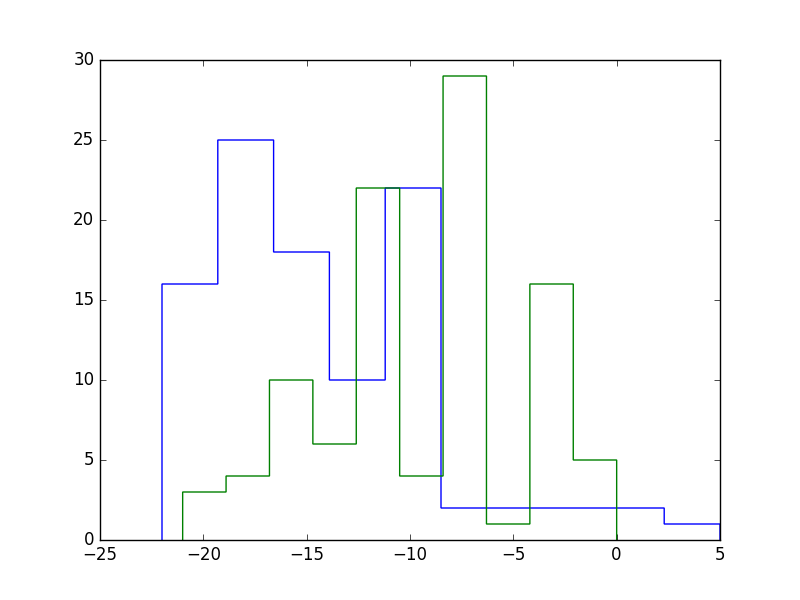
\includegraphics[width=0.5\linewidth]{Public1.png}
			
	\caption{Гистограмма выигрышей, синий - правительство, зеленый - общественность}
	\label{fig:stat1}
\end{figure}

\begin{table}[h]
	\centering
	\caption{}
			\footnotesize Статистические показатели для 100 игр\\
			\normalsize
			
	\begin{tabular}{|l|c|c|}
		\hline
		& Правительство & Общественность \\ \hline
		Среднее                                                           & -14.26        & -9.46          \\ \hline
		\begin{tabular}[c]{@{}l@{}}Стандартное \\ отклонение\end{tabular} & 5.34          & 4.66           \\ \hline
		Ассиметрия                                                        & 1.1           & -0.041         \\ \hline
		Эксцесс                                                           & 1.37          & -0.37          \\ \hline
	\end{tabular}
\end{table}

Согласно полученным результатам легко видеть, что подобный набор стратегий
невыгоден обеим сторонам, к тому же правительству из-за более <<мягкого>> подхода
<<более невыгодно>>.

Рассмотрим случай, когда правительство на последнем шаге может отступить от оптимальной для обоих игроков стратегии $(L,L)$.

Зададим распределение вероятностей выбора данной стратегии для каждого из двух игроков:
 \begin{gather*}
 	q^g = \left[ 0; 0; 0; 0; 0; 0; 0.3 \right], \\
 	q^p = \left[ 0; 0; 0; 0 \right].
 \end{gather*}


\begin{figure}[h]
	

		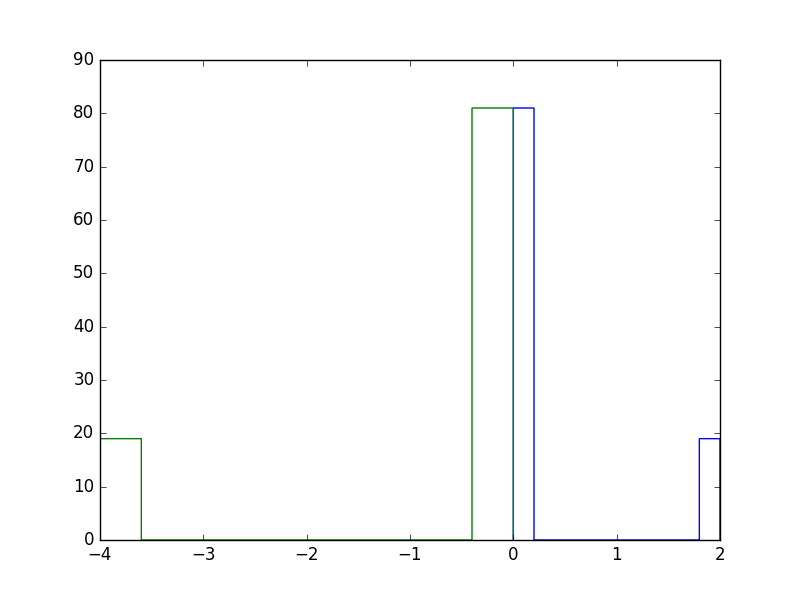
\includegraphics[width=0.5\linewidth]{Public.png}
	\centering	
	\caption{Гистограмма выигрышей, синий - правительство, зеленый - общественность}
	\label{fig:stat}
\end{figure}

\begin{table}[h]
	\centering
		\caption{}
		\footnotesize Статистические показатели для 100 игр\\
		\normalsize
	\begin{tabular}{|l|l|l|}
		\hline
		& Правительство & \multicolumn{1}{c|}{Общественность} \\ \hline
		Среднее                                                           & 0.39        & -0.78                         \\ \hline
		\begin{tabular}[c]{@{}l@{}}Стандартное \\ отклонение\end{tabular} & 0.78         & 1.56                          \\ \hline
		Ассиметрия                                                        & 1.6          & -1.11                          \\ \hline
		Эксцесс                                                           & 0.58        & 0.58                        \\ \hline
	\end{tabular}
\end{table}

Данная стратегия является выигрышной для правительства, если общественность не ожидает подобного хода под конец действия срока правительства.

Рассмотрим случай, когда общественность доверяет правительству и почти уверенно, что оно не может поднять уровень инфляции к окончанию срока своего правления.

Зададим распределение вероятностей выбора данной стратегии для каждого из двух игроков:
 \begin{gather*}
 	q^g = \left[ 0; 0; 0; 0; 0; 0; 0.3 \right], \\
 	q^p = \left[ 0; 0; 0; 0.15 \right].
 \end{gather*}
	\begin{figure}[h]
		
\centering
				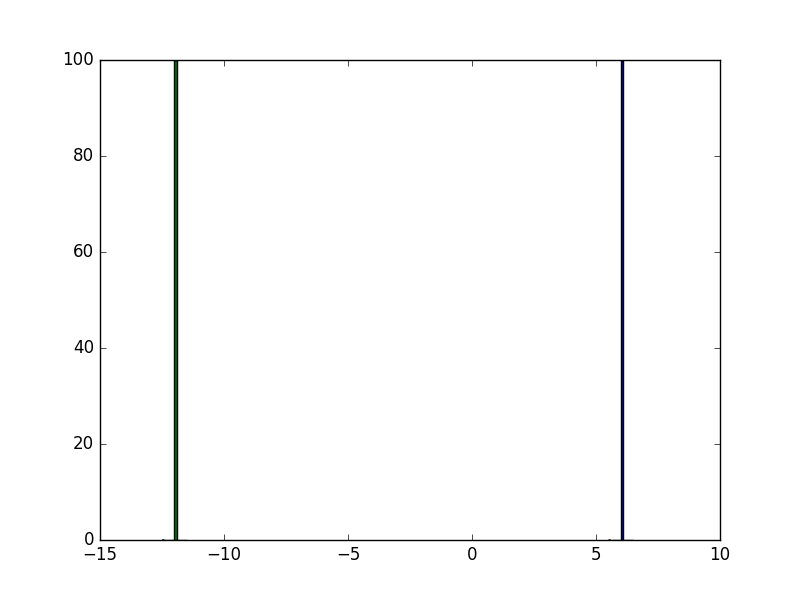
\includegraphics[width=0.5\linewidth]{Public2.png}
		
		\caption{Гистограмма выигрышей, синий - правительство, зеленый - общественность}
		\label{fig:stat2}
	\end{figure}
	\begin{table}[h]
		\centering
			\caption{}
			\footnotesize Статистические показатели для 100 игр\\
			\normalsize
 \begin{tabular}{|l|c|c|}
 	\hline
 	& Правительство & Общественность \\ \hline
 	Среднее                                                           & -0.9          & -2.18          \\ \hline
 	\begin{tabular}[c]{@{}l@{}}Стандартное \\ отклонение\end{tabular} & 3          & 2.58           \\ \hline
 	Ассиметрия                                                        & -1.16           & -0.68          \\ \hline
 	Эксцесс                                                           & -0.06          & -0.95           \\ \hline
 \end{tabular}
	\end{table}
	
Легко видеть, что данная стратегия однозначно ухудшает позицию правительства, но так же не выгодна общественности.

Рассмотрим случай, когда общественность не доверяет правительству и почти уверенно, что оно повысит уровень инфляции к окончанию срока своего правления.
 Зададим распределение вероятностей выбора данной стратегии для каждого из двух игроков:
 \begin{gather*}
 	q^g = \left[ 0; 0; 0; 0; 0; 0; 0.3 \right], \\
 	q^p = \left[ 0; 0; 0; 0.8 \right].
 \end{gather*}
 	\begin{figure}[h]
 		\centering
 			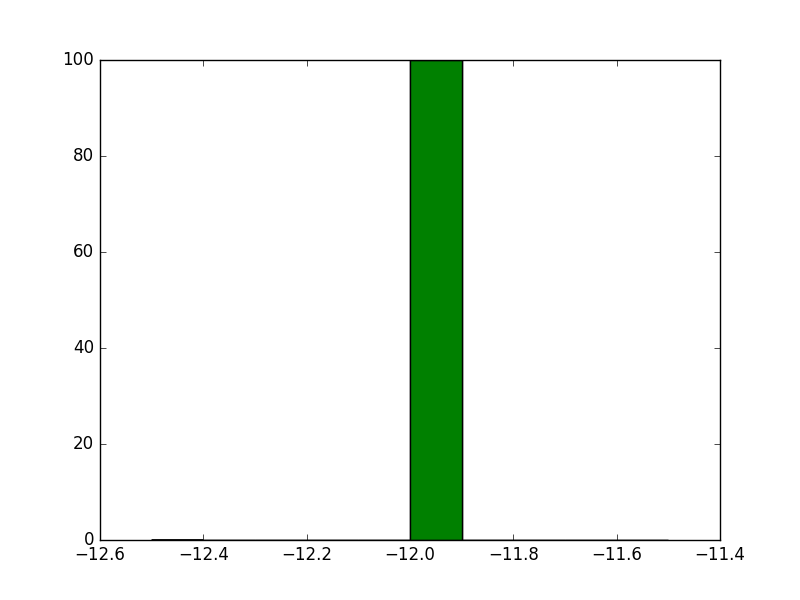
\includegraphics[width=0.5\linewidth]{Public3.png}
 		\caption{Гистограмма выигрышей, синий - правительство, зеленый - общественность}
 		\label{fig:stat3}
 	\end{figure}
 	
 	\begin{table}[h]
 		\centering	\caption{}
 		\footnotesize Статистические показатели для 100 игр\\
 		\normalsize
 	 \begin{tabular}{|l|c|c|}
 	 	\hline
 	 	& Правительство & Общественность \\ \hline
 	 	Среднее                                                           & -4.8          & -4.62          \\ \hline
 	 	\begin{tabular}[c]{@{}l@{}}Стандартное \\ отклонение\end{tabular} & 2.99          & 2.65           \\ \hline
 	 	Ассиметрия                                                        & 1.18           & 0.54          \\ \hline
 	 	Эксцесс                                                           & -0.12          & -1.15           \\ \hline
 	 \end{tabular}
 	\end{table}	
Данная стратегия является равносильно невыгодна для обоих игроков.
 
В связи с полученными результатами можно сделать вывод, что если правительство
имеет больше шагов на временных шкалах, то ей имеет смысл отклонится от
оптимальной по Парето стратегии $(L, L)$ и повысить уровень инфляции под конец
срока своего правления, так как даже если общественность будет ожидать такого
хода, то с целью минимизировать свои потери не будет повышать индексирование
заработной платы заранее. Естественно если правительство захочет заручиться
поддержкой общественности на следующих выборах, то такой ход с её стороны будет
сродни <<политическому самоубийству>>.

\subsection{Анализ устойчивости стратегий в модели профсоюз~--- монополист}
Положим матрицу выигрышей в соответствии с~\ref{table:firm} следующим образом:
\begin{table}[h]
	
	\centering
	\caption{}
	\footnotesize Матрица выигрышей соответствующая~(\ref{table:firm})\\
	\normalsize
\begin{tabular}{|l|l|c|c|}
	\hline
	\multicolumn{2}{|l|}{\multirow{2}{*}{}} & \multicolumn{2}{l|}{Профсоюз} \\ \cline{3-4} 
	\multicolumn{2}{|l|}{}                  & L            & H              \\ \hline
	\multirow{2}{*}{Фирма}        & L       & 3, 1         & 2, 3.9         \\ \cline{2-4} 
	& H       & 7, 4         & -3, 7          \\ \hline
\end{tabular}
	\label{table:mono:ex}
\end{table}\\
Для нахождения равновесия по Нэшу посчитаем следующее: \\
Фирма
	$$ L:  3\alpha + 2(1-\alpha)=\alpha + 2$$
	$$ H: 7\alpha - 3(1-\alpha)=10\alpha - 3$$
	$$10\alpha - 3 = \alpha+2 $$
	$$\alpha = \frac{5}{9} $$
Профсоюз	
	 $$L: \beta + 4(1-\beta)=-3\beta + 4$$
	 $$H: 3.9\beta + 7(1-\beta)=-3.1\beta +7$$
	$$0.1\beta  = 3 $$
	$$\beta = 30 $$
Следовательно равновесием по Нэшу будет стратегия $L,H$.

В каждом столбце матрицы фирмы найдем максимальный элемент. 
Зgтем в каждой строке матрицы профсоюза выберем наибольший элемент.
Платежная матрица фирмы:
\begin{table}[h]
	\centering
	\begin{tabular}{|l|l|}
		\hline
		3, 1 & \textbf{2, 3.9}  \\ \hline
		\textbf{7}, 4 & -3, \textbf{7} \\ \hline
	\end{tabular}
\end{table}\\
Оптимальной по Парето будет стратегия $(H,L)$. Далее полагаем $r^f= 4 $ (количество ходов фирмы за одну игру),
$r^p= 3$ (количество ходов профсоюза). 

 Рассмотрим случай, когда оба игрока стараются следовать равновесной стратегии
 по Нэшу.  Зададим распределение вероятностей выбора первой стратегии для
 каждого из двух игроков:
 \begin{gather*}
 	q^f = \left[ 0.9; 0.9; 0.9; 0.9 \right], \\
 	q^p = \left[ 0.1; 0.1; 0.1 \right].
 \end{gather*}

 	\begin{figure}[h]
 		\centering
 		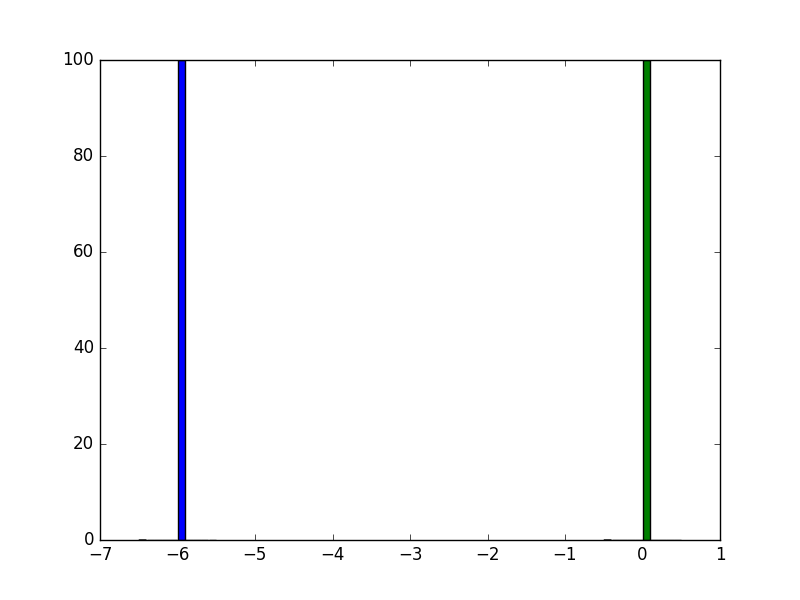
\includegraphics[width=0.5\linewidth]{Public4.png}
 		\caption{Гистограмма выигрышей, синий - фирма, зеленый - профсоюз}
 		\label{fig:stat4}
 	\end{figure}
 	
 	\begin{table}[h]
 		\centering
 			\caption{}
 			\footnotesize Статистические показатели для 100 игр\\
 			\normalsize
 		 \begin{tabular}{|l|c|c|}
 		 	\hline
 		 	& Фирма & Профсоюз\\ \hline
 		 	Среднее                                                           & 69.02          & 47.84          \\ \hline
 		 	\begin{tabular}[c]{@{}l@{}}Стандартное \\ отклонение\end{tabular} & 18.1          & 8.19           \\ \hline
 		 	Ассиметрия                                                        & -1.04           & 0.017          \\ \hline
 		 	Эксцесс                                                           & 0.25         & 0.69           \\ \hline
 		 \end{tabular}
 	\end{table}
 	
\newpage
 Рассмотрим случай, когда профсоюз пытается увеличивать зарплату, на своём
 последнем шаге, а фирма для выхода из нерентабельного положения сокращает
 количество сотрудников.  Зададим распределение вероятностей выбора данной
 стратегии для каждого из двух игроков:
 \begin{gather*}
 	q^f = \left[ 0.9; 0.9; 0.9; 0.1 \right], \\
 	q^p = \left[ 0.1; 0.1; 0.9 \right].
 \end{gather*}
 
 \begin{figure}[h]
 	\centering
 	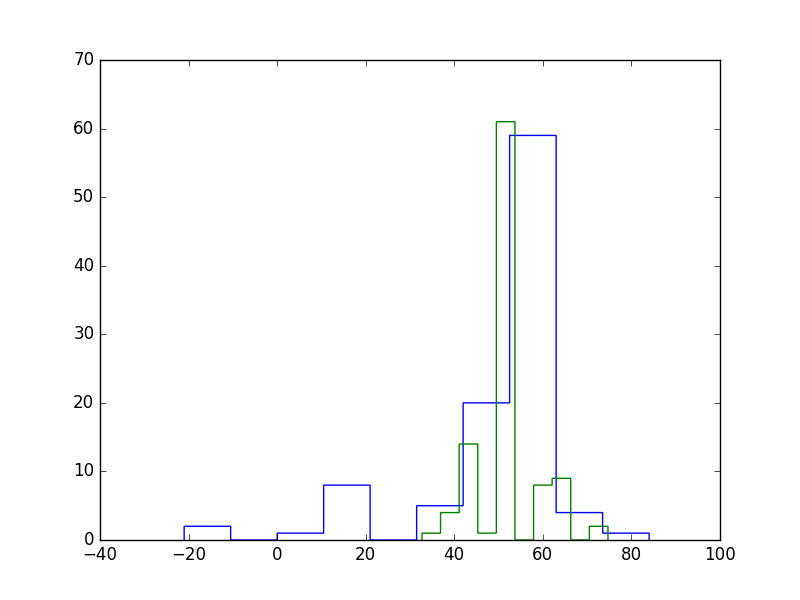
\includegraphics[width=0.5\linewidth]{Public5.png}
 	\caption{Гистограмма выигрышей, синий - фирма, зеленый - профсоюз}
 	\label{fig:stat5}
 \end{figure}
 
 \begin{table}[h]
 	\centering
 		\caption{}
 		\footnotesize Статистические показатели для 100 игр\\
 		\normalsize
  \begin{tabular}{|l|c|c|}
  	\hline
  	& Фирма & Профсоюз\\ \hline
  		Среднее                                                           & 50.48      &  51.1                        \\ \hline
 		\begin{tabular}[c]{@{}l@{}}Стандартное \\ отклонение\end{tabular} & 17.18        &  7.17                          \\ \hline
 		Ассиметрия                                                        & -2.02          &0.57                          \\ \hline
 		Эксцесс                                                           & 5.21        & 1.44                        \\ \hline
 	\end{tabular}
 \end{table}
Такая стратегия незначительно улучшит позиции профсоюза, но заметно пошатнет позицию фирмы.
\newpage
 Рассмотрим случай, когда профсоюз увеличит зарплату во второй раз и вернется к
 оптимальной стратегии на третий период.  Зададим распределение вероятностей
 выбора данной стратегии для каждого из двух игроков:
 \begin{gather*}
 	q^f = \left[ 0.9; 0.9; 0.1; 0.9 \right], \\
 	q^p = \left[ 0.1; 0.9; 0.1 \right].
 \end{gather*}
 \begin{figure}[h]
 	\centering
 	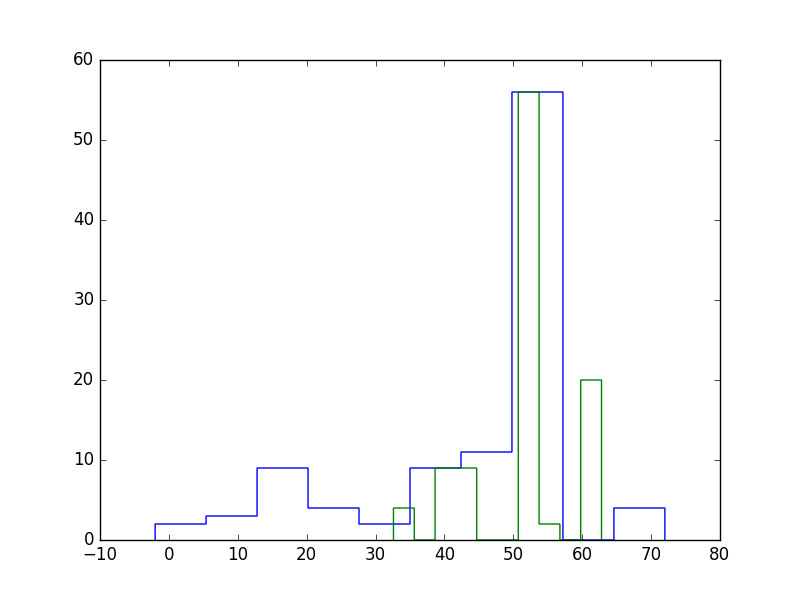
\includegraphics[width=0.5\linewidth]{Public6.png}
 	\caption{Гистограмма выигрышей, синий - фирма, зеленый - профсоюз}
 	\label{fig:stat6}
 \end{figure}
 
 \begin{table}[h]
 	\centering
 		\caption{}
 		\footnotesize Статистические показатели для 100 игр\\
 		\normalsize
  \begin{tabular}{|l|c|c|}
  	\hline
  	& Фирма & Профсоюз\\ \hline
  		Среднее                                                           & 43.06      &  50.64                        \\ \hline
 		\begin{tabular}[c]{@{}l@{}}Стандартное \\ отклонение\end{tabular} & 14.47        &  7.38                          \\ \hline
 		Ассиметрия                                                        & -1.06          &-0.29                          \\ \hline
 		Эксцесс                                                           & 1.30       &0.09                        \\ \hline
 	\end{tabular}
 \end{table}
 
 Снова таки разовая акция поднятия зарплат даёт профсоюзу незначительный выигрыш, но фирма при этом проигрывает относительно много больше, чем выигрывает профсоюз.

 Рассмотрим случай, когда профсоюз поднимает на втором своём ходе зарплату, но
 не опускает его вплоть до конца игры. Зададим распределение вероятностей
 выбора этой стратегии для каждого из двух игроков:
  \begin{gather*}
  	q^f = \left[ 0.9; 0.9; 0.1; 0.2 \right], \\
  	q^p = \left[ 0.1; 0.9; 0.8 \right].
  \end{gather*}
  \begin{figure}[h]
  	\centering
  	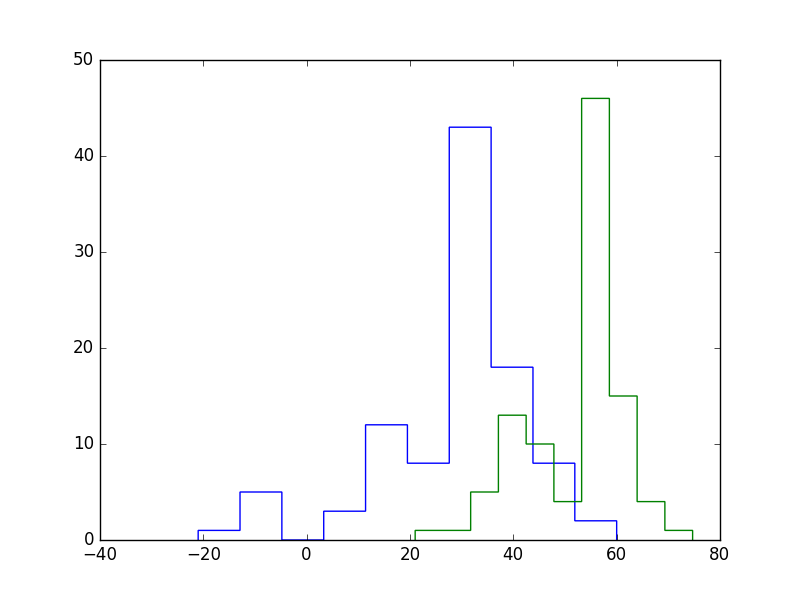
\includegraphics[width=0.5\linewidth]{Public7.png}
  	\caption{Гистограмма выигрышей, синий - фирма, зеленый - профсоюз}
  	\label{fig:stat7}
  \end{figure}
  
  \begin{table}[h]
  	\centering
  		\caption{}
  		\footnotesize Статистические показатели для 100 игр\\
  		\normalsize
   \begin{tabular}{|l|c|c|}
   	\hline
   	& Фирма & Профсоюз\\ \hline
   		Среднее                                                           & 30.37     &  51.37                        \\ \hline
  		\begin{tabular}[c]{@{}l@{}}Стандартное \\ отклонение\end{tabular} & 13.64        &  8.99                          \\ \hline
  		Ассиметрия                                                        & -1.36         &-0.53                          \\ \hline
  		Эксцесс                                                           & 2.74       & 0.8                        \\ \hline
  	\end{tabular}
  \end{table}

  \newpage
Фирма снова теряет в относительных деньгах, в то время как профсоюз только
незначительно увеличивает своё положение.  Разумно с точки зрения фирмы сделать
предложение профсоюзу не менять уровень зарплат с оптимального, а взамен
отплачивать разным видом бонусов. Тогда функция полезности изменится для обоих
игроков на равную величину. Фирме стоит подобрать эту величину бонусов так,
чтобы остаток между её оптимальным выигрышем после вычитания бонусов был чем-то
средним между собственными выигрышами, когда профсоюз устанавливает высокий
уровень зарплат и низкий.
